\chapter{手法}


\section{第一原理計算}
第一原理計算とは, シュレディンガー方程式を精確に解いて, 原子の種類だけから電子構造を求め, 様々な物性を予測する計算である. 


\section{VASP}
VASP (Vienna Ab-initio Simulation Package) は, 密度汎関数理論による平面波・擬ポテンシャル法を用いた第一原理計算プログラムパッケージである. 密度汎関数理論とは電子系等のエネルギーなどの物性は電子密度から計算できるという理論である. 擬ポテンシャル法とは原子の内殻電子を除いた価電子だけを考慮する手法であり, 全電子を計算するフルポテンシャル法に比べ比較的高速な計算が可能となるため, 擬ポテンシャル法であっても十分な精度で計算ができる.
VASP の計算には, 計算条件が記述された INCAR, 計算モデルの構造が記述された POSCAR, 原子情報が記述された POTCAR, 計算精度を司る k-mesh が記述された KPOINTS の 4 種類の入力ファイルを使用し計算を行う. その後, 計算モデル内における原子の安定位置やフォース, 系の全体エネルギー等が記述された OUTCAR 等を出力する.


\section{計算モデル}
\subsection{周期的境界条件}
VASP で計算を行う場合, 平面波を用いた第一原理計算が行われるため, 無限周期の固体を考えなければならないが計算モデル内の原子が増えるにつれ計算時間も増えるため, 無限周期のモデルの計算を行うことはできない. そこで図\ref{fig2.1} のように同じモデルが全方向に無限に隣接したようなモデルを考える. このモデルであれば, 無限周期の固体と見なせるため平面波を考慮することができる. このような計算条件を周期的境界条件という.

\begin{figure}[htbp]
	\begin{center}
		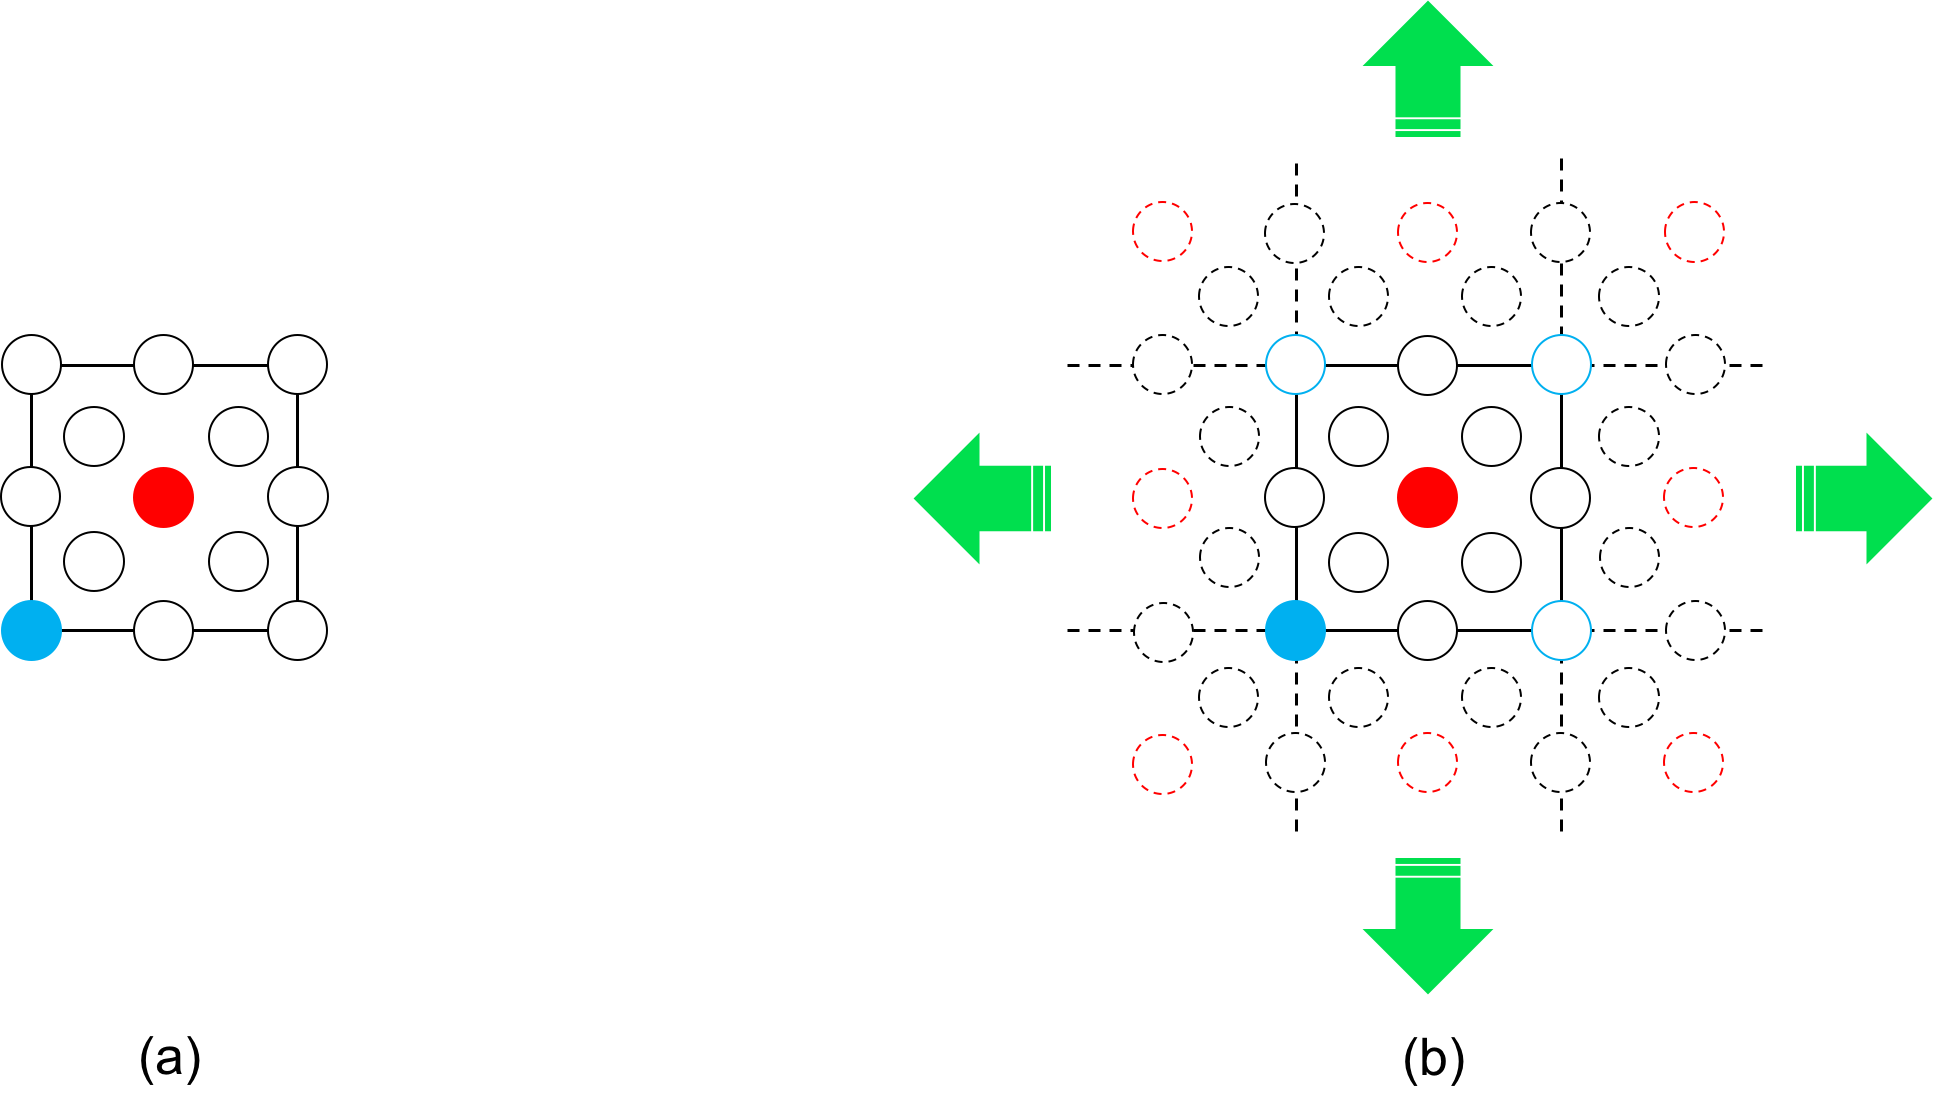
\includegraphics[width=130mm]{../method/cnd.png}
		\caption{(a) 周期的境界条件を考慮しないモデルの模式図.(b) 周期的境界条件を考慮したモデルの模式図.実線部分は計算モデル,破線部分は隣接した計算モデルを表している.}
		\label{fig2.1}
	\end{center}
\end{figure}


\subsection{ Small Cluster}

清原らは, L1$_2$ クラスターを hcp 構造に強引に導入すると, 図\ref{fig2.2} の (a), (b) のように縦方向と横方向の 2 つに分裂した集団が生成すると予測している\cite{kiyohara}. このサイズは実験的には奥田らが報告しているクラスターサイズに近い\cite{okuda}. 

\begin{figure}[htbp]
	\begin{center}
		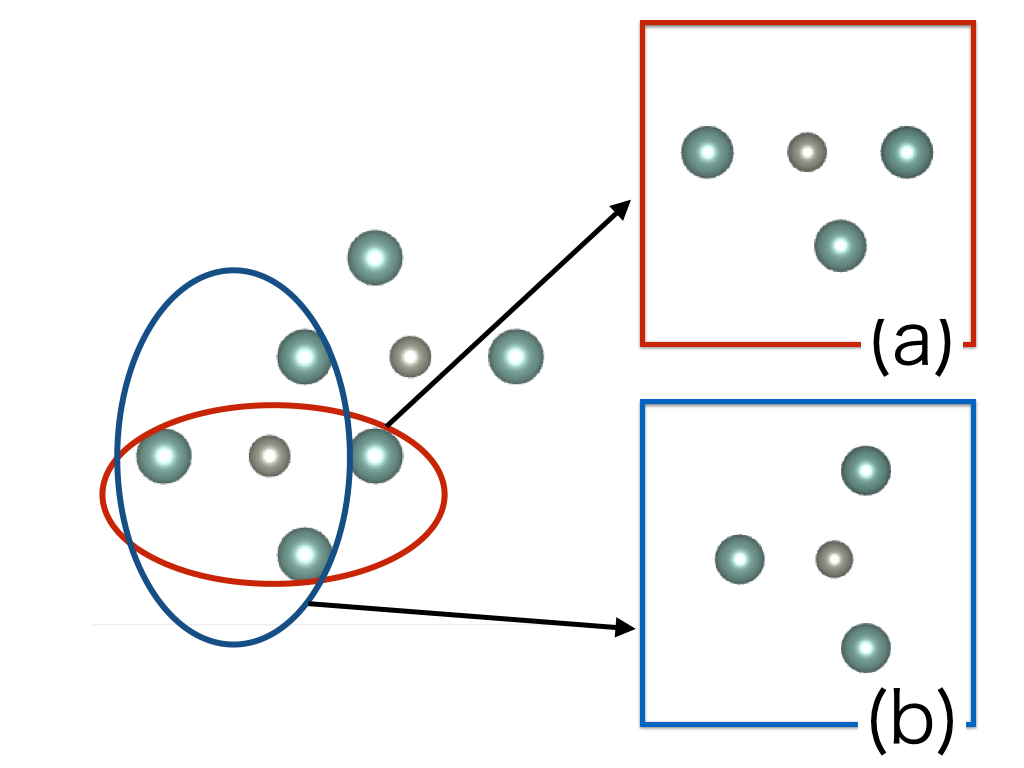
\includegraphics[width=50mm]{../method/MiniCluster.png}
		\caption{Small Cluster の模式図.}
		\label{fig2.2}
	\end{center}
\end{figure}


これらの集団を 1層12原子として, 6層の hcp-Mg 結晶に導入したモデルについて検証した. 系全体のエネルギーを第一原理計算により求めた結果, 表 2.1のような結果が得られた. この計算から, (a) のモデルのほうが (b) のモデルに比べてエネルギーの値が低く, 安定であるという結果が得られた. 今回, 本研究では (a) を Small Cluster とした. 

\begin{table}[htb]
\caption{クラスターを分割した時のエネルギー.}
  \begin{center}
    \begin{tabular}{|l|c|c|c|c|c|} \hline
 分割方法 & エネルギー [eV] \\ \hline
   (a) & -131.973930\\
\hline
   (b) & -131.730936\\
\hline
    \end{tabular}
  \end{center}
\end{table}

\subsection{ L1$_2$ クラスターおよび Small Cluster の導入}

第一原理計算では周期的境界条件が考慮されるため, 図\ref{fig2.3}に示す slub モデルが無限に隣接したようなモデルを考えなければならない. そのモデルでは Small Cluster を L1$_2$ クラスターから離していく先にも別の L1$_2$ クラスターが存在する. よって, その L1$_2$ クラスターとの相互作用の影響が及ばない距離をとるサイズで計算する必要がある. 

本研究では初めに, Small Cluster と L1$_2$ クラスターの相互作用を調べるため, 計算に最低限必要であると考えられる 図\ref{fig2.3} に示す 18層の slub モデルで計算をおこなった. L1$_2$ クラスターから [0001] 方向に 1層ずつ離した位置に Small Cluster を挿入し, VASP を用いて第一原理計算をおこない, 構造緩和したエネルギーを求めた.しかし, 18層では Small Cluster と L1$_2$ クラスターの距離を 8層以上離した計算ができなかった.


そこで, 18層の slub モデルを [0001] 方向に拡張した 24層の slub モデルを構築し, 同様にして計算をおこなった.

\begin{figure}[H]
	\begin{center}
		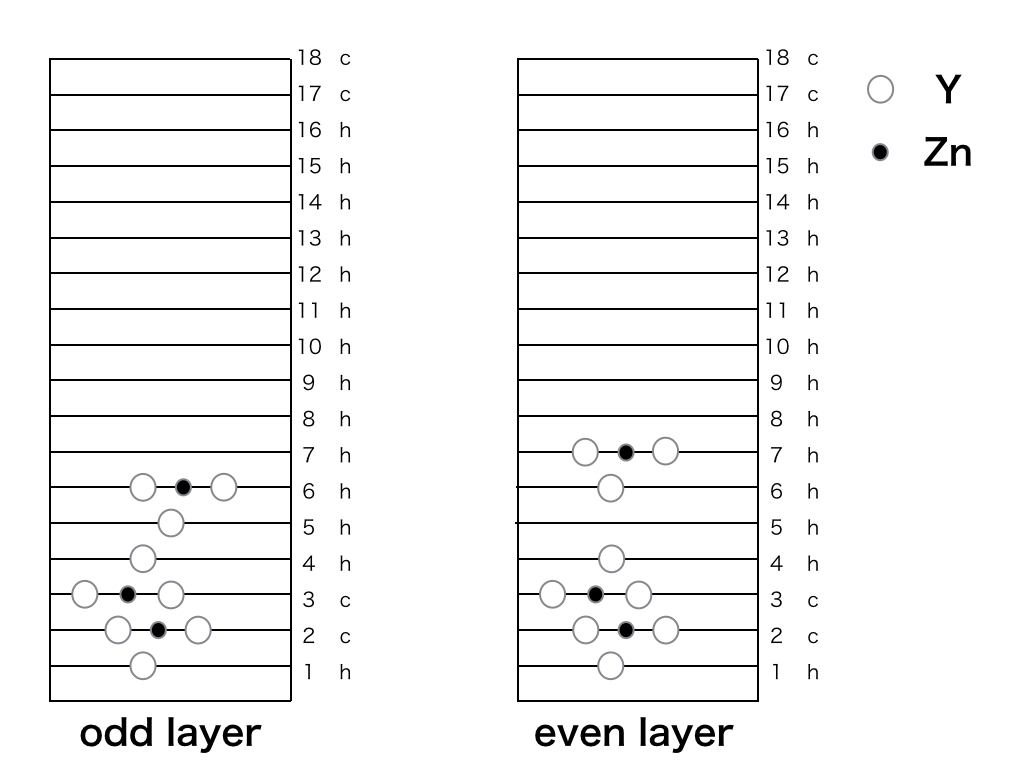
\includegraphics[width=100mm]{../method/small_cluster_slab18.png}
		\caption{slub モデルの模式図.}
		\label{fig2.3}
	\end{center}
\end{figure}


\subsection{ Small Cluster および 空孔の導入}
空孔とクラスターを含んだ Mg 結晶の安定性を検証するために, Small Cluster の周りに空孔を配置した. 図\ref{fig2.4} で表したように, 空孔を Small Cluster の [0001] 方向の a, b, c の位置に空孔を挿入した.

\begin{figure}[htbp]
	\begin{center}
		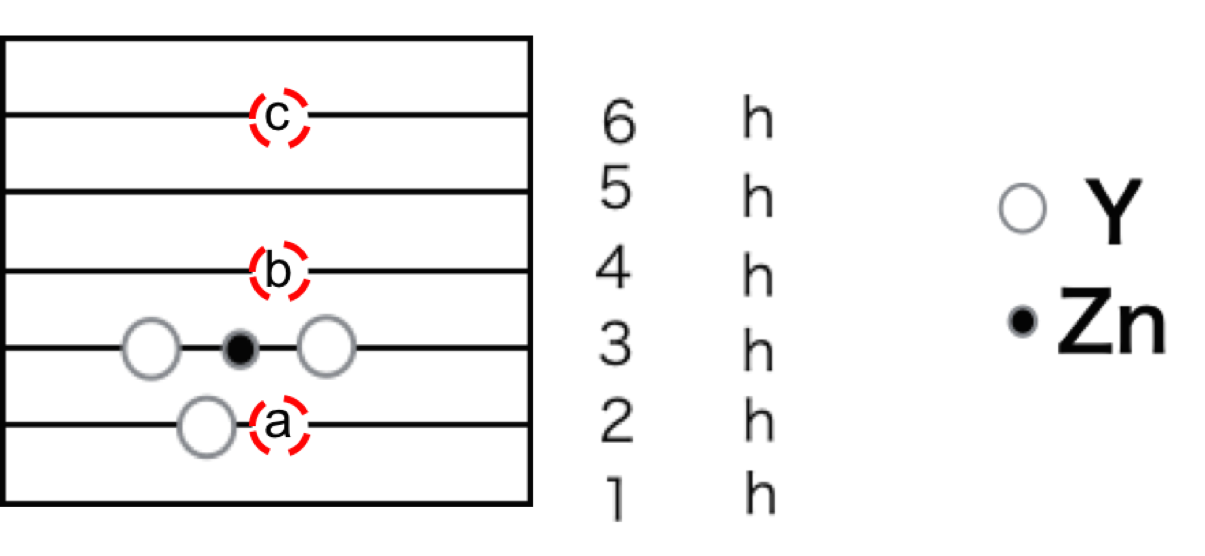
\includegraphics[width=100mm]{../method/vacancyposition.png}
		\caption{空孔の挿入位置の模式図.}
		\label{fig2.4}
	\end{center}
\end{figure}



